\chapter{Systemarchitektur}

\section{Überblick}
\begin{itemize}
    \item \textbf{Gesamtsystem:} Geben Sie eine Übersicht über die gesamte Systemarchitektur, einschließlich App, API und Datenbanken.
    \item \textbf{Hauptkomponenten:} Beschreiben Sie die Hauptkomponenten des Systems und deren Interaktionen.
    \item \textbf{Datenfluss:} Erläutern Sie den Datenfluss innerhalb des Systems vom Fingerprint-Sammeln bis zur Raumvorhersage.
\end{itemize}

\section{Datenbankstruktur}

Es wurde eine relationale Datenbank gewählt, da viele Einträge wie Räume und Router mehrfach vorkommen und so die größe der Datenbank nicht linear wächst mit jeder neuen Messung.

Die entwickelte Datenbankstruktur besteht aus vier zentralen Tabellen: \textit{rooms}, \textit{measurements}, \textit{routers} und \textit{measurement\_router}. Diese Struktur wurde gewählt, um eine effiziente und flexible Speicherung sowie Verwaltung der für die Raumbestimmung erforderlichen Daten zu gewährleisten. Die einzelnen Tabellen und deren Beziehungen sind in Abbildung \ref{fig:database-structure} dargestellt.

\begin{figure}[h]
    \centering
    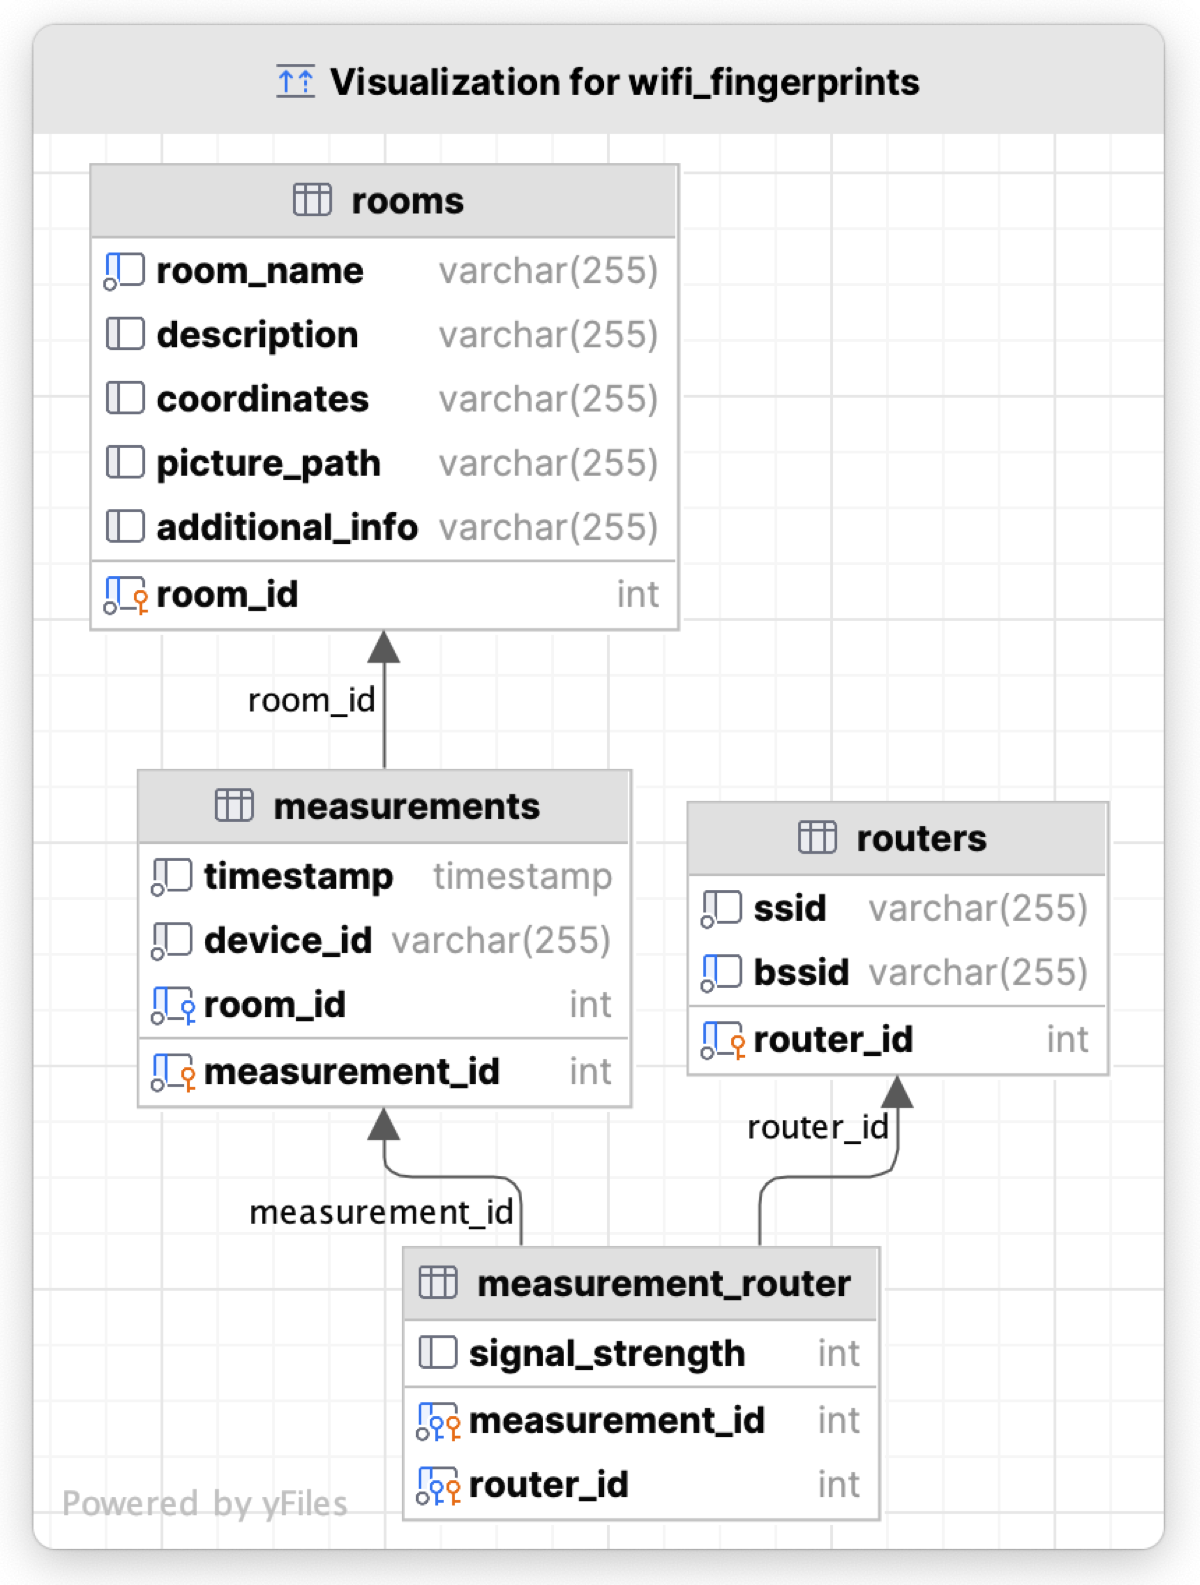
\includegraphics[width=0.3\textwidth]{images/database_strucure.png}
    \caption{Datenbankstruktur}
    \label{fig:database-structure}
\end{figure}

\begin{figure}
    \centering
    \begin{tikzpicture}[
        table/.style={rectangle split, rectangle split parts=6, draw, rounded corners, text centered, minimum height=4em, minimum width=12em, inner sep=2pt},
        link/.style={draw, -{Latex[length=3mm]}, thick},
        reversedlink/.style={draw, {Latex[length=3mm]}-, thick},
        every node/.style={font=\small},
        nodes in empty cells
    ]

    % Matrix
    \matrix (m) [matrix of nodes, row sep=2cm, column sep=2cm, nodes={table}, 
                 column 1/.style={anchor=center}, 
                 column 2/.style={anchor=center}] {
        \node[table, rectangle split parts=7] (rooms) {
            \textbf{rooms}
            \nodepart{two} room\_id : int
            \nodepart{three} room\_name : varchar(255)
            \nodepart{four} description : varchar(255)
            \nodepart{five} coordinates : varchar(255)
            \nodepart{six} picture\_path : varchar(255)
            \nodepart{seven} additional\_info : varchar(255)
        }; &
        \node[table, rectangle split parts=4] (routers) {
            \textbf{routers}
            \nodepart{two} router\_id : int
            \nodepart{three} ssid : varchar(255)
            \nodepart{four} bssid : varchar(255)
        }; \\
        \node[table, rectangle split parts=5] (measurements) {
            \textbf{measurements}
            \nodepart{two} measurement\_id : int
            \nodepart{three} timestamp : timestamp
            \nodepart{four} device\_id : varchar(255)
            \nodepart{five} room\_id : int
        }; &
        \node[table, rectangle split parts=4] (measurement_router) {
            \textbf{measurement\_router}
            \nodepart{two} signal\_strength : int
            \nodepart{three} measurement\_id : int
            \nodepart{four} router\_id : int
        }; \\
    };

    % Links
    \draw[link] (measurement_router.north) -- (routers.south);
    \draw[link] (measurement_router.west) -| ([xshift=-1.5cm]measurement_router.west) |- (measurements.east);
    \draw[link] (measurements.north) -- (rooms.south);

    \end{tikzpicture}
    \caption{Diagramm der Datenbanktabellen und ihrer Beziehungen}
    \label{fig:database-diagram}
\end{figure}


\subsection{Tabelle \textit{rooms}}

Die Tabelle \textit{rooms} speichert Informationen über alle aufgenommenen Räume. Sie enthält die folgenden Felder:
\begin{itemize}
    \item \textit{room\_id}: Primärschlüssel, der automatisch inkrementiert wird.
    \item \textit{room\_name}: Name des Raumes, der eindeutig sein muss.
    \item \textit{description}: Beschreibung des Raumes.
    \item \textit{coordinates}: Koordinaten des Raumes.
    \item \textit{picture\_path}: Pfad zu einem Bild des Raumes.
    \item \textit{additional\_info}: Weitere Informationen zum Raum.
\end{itemize}

Die Felder \textit{description}, \textit{coordinates}, \textit{picture\_path} und \textit{additional\_info} sind vorhanden, da die Datenbank auch auf mobilen Geräten läuft und die App diese Daten speichert. Dies ermöglicht eine umfassende Dokumentation und einfache Identifikation der Räume.

\subsection{Tabelle \textit{measurements}}

In der Tabelle \textit{measurements} werden alle Messungen gespeichert. Die Felder umfassen:
\begin{itemize}
    \item \textit{measurement\_id}: Primärschlüssel, der automatisch inkrementiert wird.
    \item \textit{timestamp}: Zeitstempel der Messung.
    \item \textit{device\_id}: Kennung des Geräts, das die Messung durchgeführt hat.
    \item \textit{room\_id}: Fremdschlüssel, der auf die \textit{room\_id} in der Tabelle \textit{rooms} verweist.
\end{itemize}

Bei der Hinzufügung einer neuen Messung wird überprüft, ob der Raum bereits existiert und gegebenenfalls hinzugefügt. Ebenso wird überprüft, ob der Router bereits in der Tabelle \textit{routers} vorhanden ist.

\subsection{Tabelle \textit{routers}}

Die Tabelle \textit{routers} enthält Informationen zu allen Routern, die bei den Messungen erfasst wurden:
\begin{itemize}
    \item \textit{router\_id}: Primärschlüssel, der automatisch inkrementiert wird.
    \item \textit{ssid}: SSID des Routers.
    \item \textit{bssid}: BSSID des Routers, die eindeutig sein muss.
\end{itemize}

Die Eindeutigkeit der BSSID wird durch einen einzigartigen Schlüssel sichergestellt. Dies ist notwendig, um sicherzustellen, dass jeder Router nur einmal in der Datenbank gespeichert wird.

\subsection{Tabelle \textit{measurement\_router}}

Die Tabelle \textit{measurement\_router} stellt die Beziehung zwischen den Messungen und den Routern dar und speichert die Signalstärke:
\begin{itemize}
    \item \textit{measurement\_id}: Fremdschlüssel, der auf die \textit{measurement\_id} in der Tabelle \textit{measurements} verweist.
    \item \textit{router\_id}: Fremdschlüssel, der auf die \textit{router\_id} in der Tabelle \textit{routers} verweist.
    \item \textit{signal\_strength}: Signalstärke, die bei der Messung erfasst wurde.
\end{itemize}

Die Primärschlüssel der Tabelle \textit{measurement\_router} bestehen aus der Kombination von \textit{measurement\_id} und \textit{router\_id}, um sicherzustellen, dass jede Kombination aus Messung und Router nur einmal gespeichert wird.

\subsection{Validierung und Vermeidung von Duplikaten}

Um zu verhindern, dass Messungen doppelt hinzugefügt werden, wird überprüft, ob bereits eine Messung mit derselben \textit{device\_id} und demselben \textit{timestamp} existiert. Dies stellt sicher, dass jede Messung einzigartig ist und keine redundanten Daten in der Datenbank gespeichert werden.

Zusammenfassend bietet die gewählte Datenbankstruktur eine robuste Grundlage für die Speicherung und Verwaltung der Daten, die für die Raumbestimmung mittels WiFi Fingerprints erforderlich sind. Die Struktur ermöglicht eine effiziente Verarbeitung und Abfrage der Daten, was für die Echtzeitanwendung in mobilen Geräten essenziell ist.

\subsection{MariaDB auf der VM}
\begin{itemize}
    \item \textbf{Datenbankdesign:} Beschreiben Sie das Design der MariaDB-Datenbank und die wichtigsten Tabellen.
    \item \textbf{Speicherung von Fingerprints:} Erklären Sie, wie Fingerprint-Daten in der MariaDB gespeichert und verwaltet werden.
    \item \textbf{Abfragen und API-Interaktion:} Diskutieren Sie die wichtigsten Abfragen und die Interaktion mit der API.
\end{itemize}

\subsection{SQLite auf den mobilen Geräten}
\begin{itemize}
    \item \textbf{Datenbankdesign:} Beschreiben Sie das Design der SQLite-Datenbank und die wichtigsten Tabellen.
    \item \textbf{Lokal gespeicherte Daten:} Erklären Sie, welche Daten lokal auf den mobilen Geräten gespeichert werden und warum.
    \item \textbf{Synchronisation mit MariaDB:} Diskutieren Sie die Mechanismen zur Synchronisation der SQLite-Daten mit der MariaDB.
\end{itemize}

\section{Implementierung der Android App (BVG Detection)}
\begin{itemize}
    \item \textbf{App-Architektur:} Geben Sie eine Übersicht über die Architektur der Android-App und deren Hauptkomponenten.
    \item \textbf{Funktionalitäten:} Beschreiben Sie die Hauptfunktionen der App, einschließlich Fingerprint-Aufnahme und Raumvorhersage.
    \item \textbf{Technologien und Bibliotheken:} Erklären Sie die verwendeten Technologien und Bibliotheken zur Implementierung der App.
\end{itemize}

\section{Implementierung der API}
\begin{itemize}
    \item \textbf{API-Design:} Die API wurde mit Flask entwickelt und dient der Verwaltung und Abfrage von WiFi-Fingerprints zur Indoor-Ortung. Die Hauptendpunkte sind:
        \begin{itemize}
            \item \texttt{/measurements} (POST): Hinzufügen eines neuen Fingerprints.
            \item \texttt{/measurements/batch} (POST): Hinzufügen mehrerer Fingerprints im Batch.
            \item \texttt{/measurements/all} (GET): Abrufen aller gespeicherten Fingerprints.
            \item \texttt{/measurements/reset} (POST): Zurücksetzen aller gespeicherten Fingerprints und zugehöriger Daten.
            \item \texttt{/measurements/predict} (POST): Vorhersage des Raumes basierend auf empfangenen WiFi-Daten.
            \item \texttt{/ping} (GET): Überprüfen, ob der Server läuft.
            \item \texttt{/measurements/room\_names} (GET): Abrufen aller Messungs-IDs mit ihren zugehörigen Raumnamen.
        \end{itemize}
        Jeder Endpunkt hat eine spezifische Funktion und dient entweder der Datenspeicherung, -abfrage oder -vorhersage.

    \item \textbf{Funktionalitäten:} Die API bietet folgende Hauptfunktionen:
        \begin{itemize}
            \item \textbf{Fingerprint-Speicherung:} Die Funktion \texttt{handle\_add\_measurement} ermöglicht das Hinzufügen eines neuen Fingerprints zur Datenbank. Hierbei werden Informationen wie Raumname, Geräte-ID, Zeitstempel und Routerdaten gespeichert.
            \item \textbf{Batch-Speicherung:} Mit der Funktion \texttt{handle\_add\_measurements\_batch} können mehrere Fingerprints in einem Schritt hinzugefügt werden, was die Effizienz bei der Datenerfassung erhöht.
            \item \textbf{Raumvorhersage:} Die Funktion \texttt{handle\_predict\_room} verwendet verschiedene Machine Learning Algorithmen (KNN, Random Forest, SVM), um basierend auf empfangenen WiFi-Daten den wahrscheinlichsten Raum vorherzusagen. Hierbei werden verschiedene Parameter wie der Algorithmus, die Anzahl der Nachbarn (k-Wert) und Gewichtungsstrategien berücksichtigt.
            \item \textbf{Datenabfrage:} Über die Endpunkte \texttt{/measurements/all} und \texttt{/measurements/room\_names} können alle gespeicherten Fingerprints sowie die zugehörigen Raumnamen abgerufen werden.
            \item \textbf{Daten-Reset:} Mit \texttt{handle\_reset\_measurements} können alle gespeicherten Fingerprints und zugehörige Daten zurückgesetzt werden, was besonders bei Testläufen nützlich ist.
        \end{itemize}

    \item \textbf{Sicherheitsaspekte:} Die API berücksichtigt verschiedene Sicherheitsaspekte, um den Schutz der Daten zu gewährleisten:
        \begin{itemize}
            \item \textbf{Authentifizierung und Autorisierung:} Um sicherzustellen, dass nur autorisierte Benutzer auf die API zugreifen und Änderungen vornehmen können, sollten Authentifizierungs- und Autorisierungsmechanismen wie API-Schlüssel oder OAuth implementiert werden. In der aktuellen Implementierung fehlt diese Funktionalität und sollte daher als zukünftige Verbesserung berücksichtigt werden.
            \item \textbf{Datenvalidierung:} Bei der Verarbeitung eingehender Anfragen wird die Integrität der Daten überprüft. Fehlende oder fehlerhafte Daten führen zu Fehlermeldungen und die Anfragen werden abgelehnt (z.B. \texttt{handle\_add\_measurement} überprüft, ob alle erforderlichen Felder vorhanden sind).
            \item \textbf{Logging und Monitoring:} Die API enthält Logging-Funktionalitäten, die Informationen über eingehende Anfragen und ausgehende Antworten protokollieren. Dies hilft bei der Überwachung der API-Nutzung und beim Debugging.
            \item \textbf{Fehlerbehandlung:} Die API behandelt verschiedene Fehlerzustände, wie z.B. das Überschreiten der Zeitlimits für Anfragen oder Netzwerkprobleme, und liefert entsprechende Fehlermeldungen an den Client.
        \end{itemize}
\end{itemize}


\section{Kommunikationsfluss zwischen App und API}
\begin{itemize}
    \item \textbf{Datenübertragung:} Erläutern Sie, wie die Datenübertragung zwischen der App und der API erfolgt.
    \item \textbf{Protokolle und Formate:} Beschreiben Sie die verwendeten Protokolle und Datenformate (z.B. JSON, HTTP).
    \item \textbf{Synchronisationsmechanismen:} Erklären Sie die Mechanismen zur Synchronisation und Datenkonsistenz zwischen App und API.
\end{itemize}

\section{Bluetooth-Datenaustausch zwischen Geräten}
\begin{itemize}
    \item \textbf{Funktionalität:} Der Bluetooth-Datenaustausch zwischen Geräten ermöglicht es, WiFi-Fingerprints direkt zwischen zwei Geräten auszutauschen, ohne eine zentrale Datenbank oder API verwenden zu müssen. Dies ist besonders nützlich, wenn eine schnelle und lokale Synchronisation der Daten erforderlich ist, beispielsweise in Umgebungen ohne Internetzugang. Die Bluetooth-Kommunikation ermöglicht es, dass Gerät A Fingerprints an Gerät B senden kann und umgekehrt. Dies erweitert die Flexibilität und Anwendungsmöglichkeiten der App erheblich.

    \item \textbf{Technische Umsetzung:} Die technische Umsetzung des Bluetooth-Datenaustauschs in der Android-App erfolgt durch die Verwendung der BluetoothAdapter- und BluetoothSocket-Klassen von Android. Der Prozess beinhaltet die folgenden Schritte:
        \begin{itemize}
            \item \textbf{Initialisierung:} Der BluetoothAdapter wird initialisiert, um das Bluetooth-Modul des Geräts zu steuern. Falls Bluetooth nicht aktiviert ist, wird der Benutzer aufgefordert, es zu aktivieren.
            \item \textbf{Paaren von Geräten:} Eine Liste der gekoppelten Bluetooth-Geräte wird angezeigt, und der Benutzer kann ein Gerät auswählen, mit dem eine Verbindung hergestellt werden soll.
            \item \textbf{Verbindung herstellen:} Die App startet einen Server-Socket (AcceptThread) auf einem Gerät, der auf eingehende Verbindungen wartet. Ein anderes Gerät kann sich mit diesem Server-Socket verbinden (ConnectThread).
            \item \textbf{Datenübertragung:} Nachdem die Verbindung hergestellt ist, wird ein ConnectedThread gestartet, der die Datenübertragung verwaltet. Die Fingerprint-Daten werden in JSON-Format konvertiert und in Blöcken über die Bluetooth-Verbindung gesendet. Der Empfang und das Zusammenfügen der Daten erfolgt ebenfalls in diesem Thread.
            \item \textbf{Verarbeitung empfangener Daten:} Die empfangenen Daten werden geparst und in die lokale SQLite-Datenbank eingefügt oder aktualisiert. Der BluetoothHelper kümmert sich um die Verarbeitung der empfangenen JSON-Daten und deren Integration in die bestehende Datenbankstruktur.
        \end{itemize}

    \item \textbf{Anwendungsfälle:} Der Bluetooth-Datenaustausch bietet mehrere Vorteile und Anwendungsfälle:
        \begin{itemize}
            \item \textbf{Schnelle lokale Synchronisation:} Ideal für Umgebungen ohne Internetzugang, da die Daten direkt zwischen den Geräten ausgetauscht werden können.
            \item \textbf{Datensicherung und -wiederherstellung:} Ein Benutzer kann seine Fingerprint-Daten auf ein anderes Gerät übertragen, um eine Datensicherung zu erstellen oder Daten wiederherzustellen.
            \item \textbf{Kollaborative Datensammlung:} Mehrere Benutzer können parallel Fingerprint-Daten sammeln und diese anschließend miteinander teilen, um eine umfassendere Datenbasis zu schaffen.
            \item \textbf{Redundanz und Ausfallsicherheit:} Durch den Austausch der Daten zwischen Geräten wird sichergestellt, dass die Daten auch bei einem Geräteausfall nicht verloren gehen.
        \end{itemize}
\end{itemize}

